\documentclass[12pt, twoside]{article}
%\documentclass[12pt, twoside]{article}
\usepackage[letterpaper, margin=1in, headsep=0.2in]{geometry}
\setlength{\headheight}{0.6in}
%\usepackage[english]{babel}
\usepackage[utf8]{inputenc}
\usepackage{microtype}
\usepackage{amsmath}
\usepackage{amssymb}
%\usepackage{amsfonts}
\usepackage[nomessages]{fp} %\FPeval{\var-name}{2*sin(pi/6)}
\usepackage{siunitx} %units in math. eg 20\milli\meter
\usepackage{yhmath} % for arcs, overparenth command
\usepackage{tikz} %graphics
\usetikzlibrary{quotes, angles, arrows, arrows.meta}
\usepackage{pgfplots}
\usepgfplotslibrary{fillbetween}
\pgfplotsset{compat=1.16}
\usepackage{graphicx} %consider setting \graphicspath{{images/}}
\usepackage{parskip} %no paragraph indent
\usepackage{enumitem}
\usepackage{multicol}
\usepackage{venndiagram}

\usepackage{fancyhdr}
\pagestyle{fancy}
\fancyhf{}
\renewcommand{\headrulewidth}{0pt} % disable the underline of the header
\raggedbottom
\hfuzz=2mm %suppresses overfull box warnings

\usepackage{hyperref}

\fancyhead[LO]{La Scuola d'Italia / Dr.\ Huson / IB Math 12 \\* 4 November 2026}
\fancyhead[RO]{\fbox{\begin{minipage}{6cm}\footnotesize Nickname:\\[0.5cm]\end{minipage}}}
\fancyhead[LE]{\fbox{\begin{minipage}{6cm}\footnotesize Nickname:\\[0.5cm]\end{minipage}}}
\fancyfoot[C]{\thepage}

\begin{document}
\subsubsection*{3.3 Pre-Test: Trigonometric Functions}

A calculator is allowed. Give answers correct to three significant figures,
unless they are exact. Angles are in radians unless they are given in
degrees. Diagrams are not to scale.

\begin{enumerate}[itemsep=0.15cm]

%--- Problem 1: Radian measure: degrees to radians exact; radians to degrees; arc length and sector area; angle from a given area [9 marks] ---
%--- Source: Original (AA SL 3.4) ---
\item[1.] [Maximum mark: 9]

\begin{center}
\fbox{\begin{minipage}{0.6\textwidth}
\centering
arc length $l = r\theta$
\qquad
area of a sector $A = \dfrac{1}{2}r^{2}\theta$
\end{minipage}}
\end{center}

\begin{enumerate}[itemsep=0.1cm]
  \item Write $135^\circ$ in radians, as an exact multiple of $\pi$.
  \hfill [1]
  \item Convert $2.4$ radians to degrees. \hfill [2]
\end{enumerate}

\begin{minipage}[t]{0.62\linewidth}
The diagram shows a sector $AOB$ of a circle with centre $O$ and radius
$9\,\text{cm}$. The angle $A\hat{O}B = 1.2$ radians.
\end{minipage}
\hfill
\begin{minipage}[t]{0.33\linewidth}
\vspace{0pt}
\begin{tikzpicture}[scale=0.32]
  \coordinate (O) at (0,0);
  \coordinate (A) at (9,0);
  \coordinate (B) at (68.755:9);
  \draw[thick] (A) -- (O) -- (B);
  \draw[thick] (A) arc (0:68.755:9);
  \draw (1.6,0) arc (0:68.755:1.6);
  \node at (34:2.6) {\footnotesize $1.2$};
  \node[below left] at (O) {$O$};
  \node[right] at (A) {$A$};
  \node[above] at (B) {$B$};
  \node[below] at (4.5,0) {\footnotesize $9\,\text{cm}$};
\end{tikzpicture}
\end{minipage}

\begin{enumerate}[itemsep=0.1cm]
  \item[(c)] Find the length of the arc $AB$. \hfill [2]
  \item[(d)] Find the area of the sector $AOB$. \hfill [2]
  \item[(e)] A second sector of the same circle has an area of
  $60\,\text{cm}^{2}$. Find the angle of this sector, in radians.
  \hfill [2]
\end{enumerate}

\begin{tikzpicture}
  \draw (-0.6,0) rectangle (14.6,9.0);
  \foreach \y in {1,2,...,8} \draw[dotted] (0,\y)--(14.1,\y);
\end{tikzpicture}

\newpage

%--- Problem 2: Unit circle: exact values; cos given with quadrant, find sin and tan exactly; solve 2sin x + 1 = 0 on [0, 2pi] exactly [10 marks] ---
%--- Source: Original (AA SL 3.5, 3.6, 3.8) ---
\item[2.] [Maximum mark: 10]

\begin{enumerate}[itemsep=0.1cm]
  \item Write down the exact value of
  \begin{enumerate}[label=(\roman*), itemsep=0.05cm]
    \item $\cos\dfrac{3\pi}{4}$; \hfill [1]
    \item $\sin\dfrac{5\pi}{3}$; \hfill [1]
    \item $\tan\dfrac{4\pi}{3}$. \hfill [1]
  \end{enumerate}
  \item Given that $\cos\theta = -\dfrac{5}{13}$ and
  $\pi < \theta < \dfrac{3\pi}{2}$, find the exact value of
  \begin{enumerate}[label=(\roman*), itemsep=0.05cm]
    \item $\sin\theta$; \hfill [3]
    \item $\tan\theta$. \hfill [1]
  \end{enumerate}
  \item Solve the equation $2\sin x + 1 = 0$ for $0 \le x \le 2\pi$.
  Give your answers as exact multiples of $\pi$. \hfill [3]
\end{enumerate}

\begin{tikzpicture}
  \draw (-0.6,0) rectangle (14.6,12.7);
  \foreach \y in {1,2,...,13} \draw[dotted] (0,\y)--(14.1,\y);
\end{tikzpicture}

\newpage

%--- Problem 3: Graph of f(x) = 4cos(6x) + 3: period from graph; a, b, d; vertical stretch then translation gives h; describe transformations from y = cos x [10 marks] ---
%--- Source: Original (AA SL 2.11, 3.7) ---
\item[3.] [Maximum mark: 10]

The diagram shows part of the graph of $f(x) = a\cos(bx) + d$, for
$0 \le x \le \dfrac{2\pi}{3}$, where $a,\ b,\ d > 0$. The graph has a
maximum point at $(0,\ 7)$ and a minimum point at
$\left(\dfrac{\pi}{6},\ -1\right)$.

\begin{center}
\begin{tikzpicture}
\begin{axis}[
  axis lines=left,
  xlabel={$x$}, ylabel={$y$},
  xlabel style={at={(axis description cs:1,0)}, anchor=north west},
  ylabel style={at={(axis description cs:0,1)}, anchor=south east, rotate=-90},
  xmin=0, xmax=2.2, ymin=-3, ymax=8.5,
  xtick={0.2618,0.5236,0.7854,1.0472,1.3090,1.5708,1.8326,2.0944},
  xticklabels={$\frac{\pi}{12}$,$\frac{\pi}{6}$,$\frac{\pi}{4}$,$\frac{\pi}{3}$,
    $\frac{5\pi}{12}$,$\frac{\pi}{2}$,$\frac{7\pi}{12}$,$\frac{2\pi}{3}$},
  ytick={-3,-2,...,8},
  grid=major, grid style={line width=0.2pt, gray!40},
  tick label style={font=\footnotesize},
  width=12cm, height=7.2cm,
]
  \draw[thick] (axis cs:0,0) -- (axis cs:2.2,0);
  \addplot[very thick, domain=0:2.0944, samples=200] {4*cos(deg(6*x)) + 3};
  \addplot[only marks, mark=*, mark size=1.8pt] coordinates {(0,7) (0.5236,-1)};
  \node[anchor=south west, fill=white, inner sep=1pt, font=\small] at (axis cs:0.03,7.35) {$(0,\ 7)$};
  \node[anchor=north, fill=white, inner sep=1pt, font=\small] at (axis cs:0.5236,-1.35) {$\left(\frac{\pi}{6},\ -1\right)$};
\end{axis}
\end{tikzpicture}
\end{center}

\begin{enumerate}[itemsep=0.1cm]
  \item Write down the period of $f$. \hfill [1]
  \item Find the value of $a$, of $b$ and of $d$. \hfill [3]
  \item The graph of $f$ is stretched vertically with scale factor
  $\dfrac{1}{2}$, and then translated $5$ units down, to give the graph
  of $h$. Find $h(x)$ in the form $h(x) = p\cos(qx) + r$. \hfill [3]
  \item Describe fully the sequence of transformations that maps the graph
  of $y = \cos x$ onto the graph of $y = f(x)$. \hfill [3]
\end{enumerate}

\begin{tikzpicture}
  \draw (-0.6,0) rectangle (14.6,7.0);
  \foreach \y in {1,2,...,6} \draw[dotted] (0,\y)--(14.1,\y);
\end{tikzpicture}

\newpage

%--- Problem 4: Tide model D(t) = 2.5sin(0.5t) + 6: max and min depth; period; depth at t = 9; GDC window D >= 7; time of first low tide [11 marks] ---
%--- Source: Original (AA SL 3.7, 2.11) ---
\item[4.] [Maximum mark: 11]

The depth of water at the entrance to a harbour, $D$ metres, is modelled by
\[
  D(t) = 2.5\sin(0.5t) + 6, \qquad t \ge 0,
\]
where $t$ is the time in hours after midnight.

\begin{enumerate}[itemsep=0.1cm]
  \item Write down the maximum depth and the minimum depth of the water.
  \hfill [2]
  \item Find the period of $D$. \hfill [2]
  \item Find the depth of the water at 09:00. \hfill [2]
  \item A ship can enter the harbour only when the depth of the water is
  at least $7$ metres. Find the length of time between $t = 0$ and
  $t = 12$ during which the ship can enter the harbour. \hfill [3]
  \item Find the first time after midnight at which the water is at its
  minimum depth. \hfill [2]
\end{enumerate}

\begin{tikzpicture}
  \draw (-0.6,0) rectangle (14.6,13.0);
  \foreach \y in {1,2,...,12} \draw[dotted] (0,\y)--(14.1,\y);
\end{tikzpicture}

\end{enumerate}
\end{document}
